\documentclass{article}
\usepackage{graphicx} % Required for inserting images
\usepackage{lipsum}
\usepackage[margin=1in, includefoot, includehead]{geometry}
\usepackage{amsmath}
\usepackage[colorlinks=true,linkcolor=blue,urlcolor=blue]{hyperref}
\usepackage{amsfonts}
\usepackage{amssymb}
\usepackage[hidelinks]{hyperref}
\usepackage{fancyhdr}
\usepackage{minted}
\usepackage[spanish]{babel}
\addto\captionsspanish{\renewcommand{\tablename}{Tabla}}
\pagestyle{fancy}
\fancyhead{}
\fancyfoot{}
\fancyhead[R]{\myTitle}
\fancyfoot[L]{Simulación Numérica}
\fancyfoot[R]{\thepage}
\renewcommand{\footrulewidth}{1pt}
\usepackage[spanish]{babel}
\newcommand{\myTitle}{Taller 1: Promedios}
\newcommand{\myName}{González García, María}
\newcommand{\myDate}{\today}

\begin{document}

%PORTADA PRINCIPAL
\begin{titlepage}
    \begin{center}
        
\includegraphics[scale=0.17]{img/UAX.png}\\
        \huge{\textbf{Universidad Alfonso X\\ El Sabio}} \\
        [0.25in] 
        
        \textbf{\Large{Grado en Ingeniería Matemática}}\\
        \Large{Simulación Numérica}\\
    
        \line(1,0){400}\\
        [2mm]
        \textsc{\Large{\myTitle}} \\
        \line(1,0){400} \\
        [1in]
    \end{center}
    \begin{center}
        \textsc{\Large Autor:}	\\
        \myName\\
        [1in]
        \myDate
    \end{center}
\end{titlepage}

%ABSTRACT
\begin{abstract}
Este trabajo presenta el desarrollo y aplicación de herramientas estadísticas para el análisis de un conjunto de datos en el contexto de la simulación numérica. Se centra en el cálculo de parámetros estadísticos fundamentales, como el promedio, la varianza, la desviación estándar y el coeficiente de variación, a partir de funciones programada en Python.\\

Además, se realiza un estudio específico sobre el coeficiente de expansión térmica del acero, utilizando datos experimentales y aplicando los métodos estadísticos desarrollados. Para complementar el análisis, se emplean técnicas de visualización gráfica, generando histogramas que permiten evaluar la distribución de los valores y su posible ajuste a una distribución normal.\\

\hfill \textit{Palabras clave:} estadística, medidas de dispersión, coeficiente de variación, varianza, histograma.

\end{abstract}


%ÍNDICE
\newpage
\tableofcontents

%INTRODUCCIÓN
\newpage
\section{Introducción.}
\textbf{Ejercicio 1.} Cree una función en python que a partir de un conjunto de datos xi determine el valor promedio de los datos, la desviación estándar, la varianza y el coeficiente de variación.\\

\textbf{Ejercicio 2.} A partir de los datos aportados en el archivo \textit{Datos Taller 1.txt}, determine el valor promedio del coeficiente de expansión térmica del acero medido en:
$x 10^{-6} \text{ in}/(\text{in} \cdot {}^{\circ}F)$ su desviación estándar, varianza y coeficiente de variación utilizando la función realizada en el apartado anterior. Además, cree un histograma de los datos obtenidos.


%MÉTODOS Y MODELOS MATEMÁTICOS
\newpage
\section{Métodos y modelos matemáticos.}
\subsection{Modelos Estadísticos Aplicados.}
En esta sección, se presentan los modelos matemáticos utilizados para calcular los principales parámetros estadísticos del conjunto de datos. Estos modelos permiten describir la distribución de los valores, evaluar su variabilidad y obtener medidas representativas que faciliten su análisis. Se abordarán el cálculo del promedio, la varianza, la desviación estándar y el coeficiente de variación.
\subsubsection{Modelo de Promedio y Medidas de Tendencia Central.}
El \textbf{promedio} o \textbf{media aritmética} es una de las principales medidas de tendencia central utilizadas en estadística. Su propósito es representar un conjunto de datos mediante un único valor que resume el comportamiento general de la muestra o población analizada. Este parámetro es fundamental en el análisis de datos, ya que permite realizar comparaciones y establecer patrones en la distribución de los valores observados. Matemáticamente, la media aritmética se define como:

\begin{equation}
    \bar{y} = \frac{1}{N} \sum_{i=1}^{N} y_i
\end{equation}
Siendo:
\begin{itemize}
    \item $\bar{y}$ representa el promedio del conjunto de datos.
    \item $N$ es el número total de observaciones.
    \item $y_i$ son los valores individuales del conjunto de datos.
\end{itemize}
Este modelo matemático es ampliamente utilizado, ya que proporciona una referencia sobre el comportamiento general de un sistema. Sin embargo, la media aritmética puede verse afectada por \textbf{valores extremos o atípicos (outliers)}, lo que puede distorsionar su interpretación.\\

Para complementar el análisis, es habitual acompañar la media con otras medidas de tendencia central, como la \textbf{mediana} (que divide el conjunto de datos en dos partes iguales) y la \textbf{moda} (el valor más frecuente). Estas herramientas permiten obtener una visión más precisa de la distribución de los datos, minimizando el impacto de valores anómalos.

\subsubsection{Modelo de Dispersión: Varianza y Desviación Estándar.}
Para evaluar la variabilidad de un conjunto de datos respecto a su promedio, se emplean la \textbf{desviación estándar} y la \textbf{varianza}. Estas métricas permiten cuantificar el grado de dispersión de los valores, proporcionando información sobre la estabilidad y homogeneidad de los datos.\\

\noindent \textbf{Desviación estándar.}

\noindent La \textbf{desviación estándar} es la medida más utilizada para determinar la dispersión de los datos en torno a su media. Se define matemáticamente como:
\begin{equation}
    s_y = \sqrt{\frac{S_t}{n-1}}
\end{equation}
dónde $S_t$ representa la suma de los cuadrados de las diferencias entre cada dato $y_i$ y el promedio $\bar{y}$:
$$
S_t = \sum (y_i - \bar{y})^2
$$

El denominador $n-1$ se emplea debido a la \textbf{corrección de Bessel}, que ajusta la estimación cuando se trabaja con muestras finitas en lugar de poblaciones completas. Esto se debe a que, si se conoce la media aritmética y se tienen $n-1$ valores, el último dato puede determinarse de manera única. En consecuencia, un solo valor aislado no tiene dispersión, ya que su desviación estándar no puede calcularse correctamente.\\

\noindent \textbf{Varianza.}

\noindent La \textbf{varianza} es otra medida clave para cuantificar la dispersión de los datos, y se define como el cuadrado de la desviación estándar. Esta expresión indica cuánto se desvían, en promedio, los valores individuales respecto a la media.
\begin{equation}
    s_y^2 = \frac{\sum (y_i - \bar{y})^2}{n-1}
\end{equation}

No obstante, la varianza también puede calcularse sin necesidad de conocer previamente la media aritmética, mediante la siguiente fórmula alternativa:
\begin{equation}
    s_y^2 = \frac{\sum y_i^2 - \frac{(\sum y_i)^2}{n}}{n-1}
\end{equation}

Esta versión permite obtener la varianza de un conjunto de datos utilizando únicamente las sumas de los valores y los cuadrados de estos, lo cual puede ser útil en cálculos computacionales y en análisis donde la media no ha sido determinada previamente.

\subsubsection{Modelo de Variabilidad Relativa: Coeficiente de Variación.}
El \textbf{coeficiente de variación (CV)} es una medida estadística utilizada para evaluar la variabilidad relativa de un conjunto de datos con respecto a su media. El coeficiente de variación se expresa en porcentaje, lo que permite comparar la dispersión entre conjuntos de datos con magnitudes diferentes. Matemáticamente, el coeficiente de variación se define como la relación entre la desviación estándar y la media aritmética:
\begin{equation}
    CV = \left( \frac{s_y}{\bar{y}} \right) \times 100\%
\end{equation}

\noindent \textbf{Interpretación y Aplicaciones.}

El coeficiente de variación es particularmente útil cuando se necesita comparar la dispersión de distintos conjuntos de datos que tienen unidades diferentes. Un \textbf{CV alto} indica una mayor dispersión relativa en comparación con la media, mientras que un \textbf{CV bajo} sugiere una menor variabilidad en relación con la media del conjunto de datos.\\

\noindent \textbf{Limitaciones y Restricciones.}

No obstante, su interpretación carece de validez cuando la \textbf{media es nula}, pues la expresión matemática se torna indefinida, requiriendo en tales casos el uso de otras métricas, como la desviación estándar o la varianza.
\newpage

\subsection{Representación Gráfica.}
En el análisis estadístico, la representación gráfica de los datos es esencial para visualizar su distribución y comprender su comportamiento. Una de las herramientas más utilizadas para este propósito es el \textbf{histograma}, que permite observar la frecuencia con la que ocurren ciertos valores dentro de intervalos específicos. Además, cuando los datos siguen una \textbf{distribución normal}, se puede superponer una curva de densidad, facilitando la identificación de tendencias y la evaluación de la dispersión de los valores.
\subsubsection{Histograma y su Interpretación.}
El histograma es un gráfico de barras que representa la distribución de un conjunto de datos dividiendo el rango de valores en intervalos. La altura de cada barra indica la frecuencia con la que los valores caen dentro de cada intervalo. Este tipo de visualización es útil para identificar la tendencia central, la dispersión y posibles asimetrías en los datos.

Cuando un conjunto de datos sigue una \textbf{distribución normal}, la forma del histograma tiende a asemejarse a una curva simétrica en forma de campana. En estos casos, es común superponer una curva de densidad normal, la cual permite evaluar visualmente si los datos presentan una distribución aproximadamente normal.

\begin{figure}[h]
    \centering
    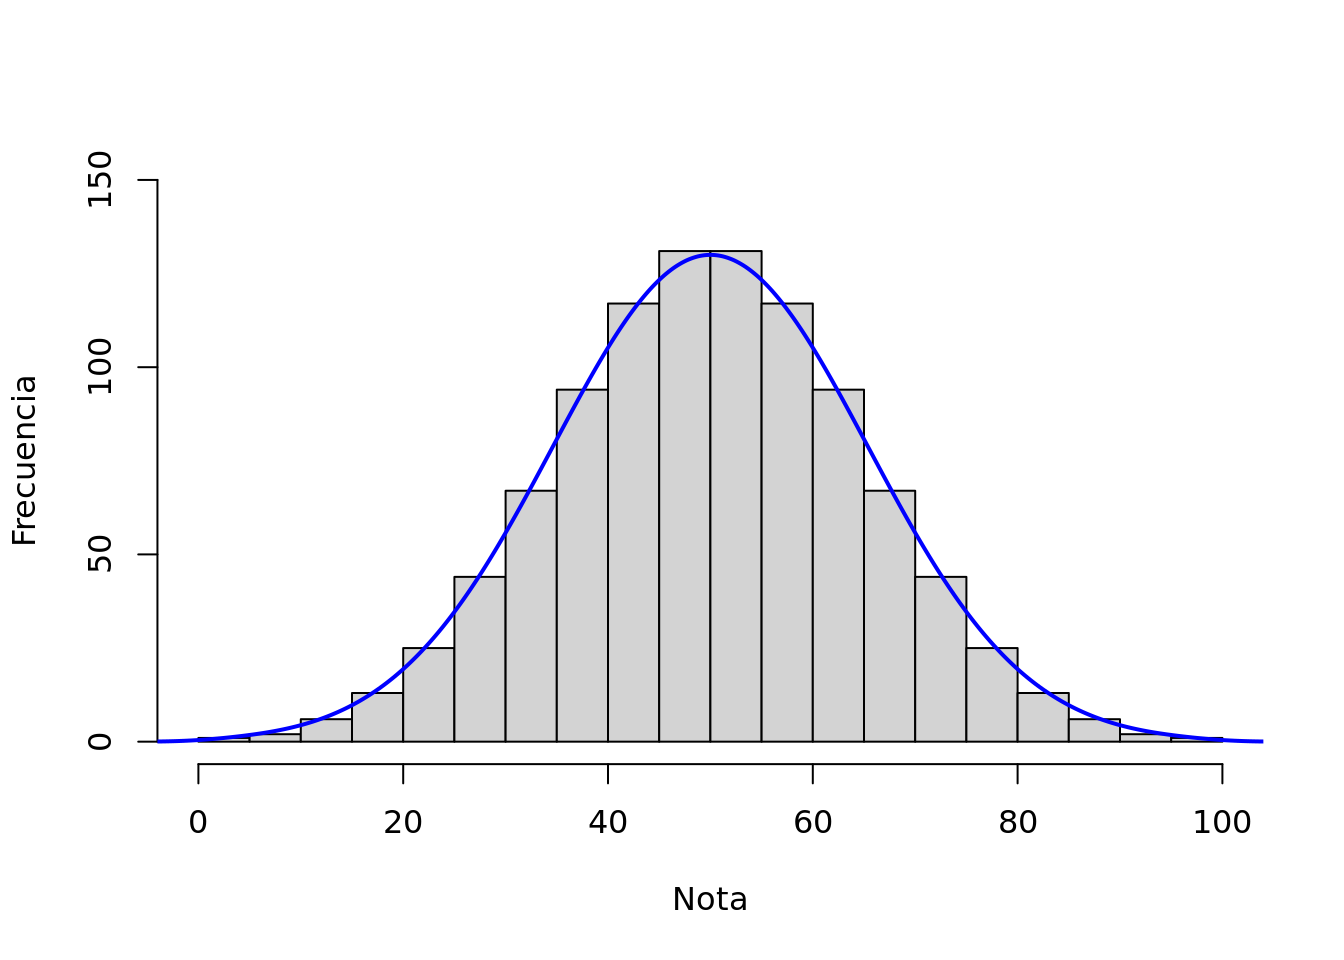
\includegraphics[width=0.5\linewidth]{img/histograma-ejemplo.png}
    \caption{Histograma de distribución normal.}
    \label{fig:hist}
\end{figure}

%RESULTADOS
\newpage
\section{Resultados.}
A partir del análisis estadístico de los datos del coeficiente de expansión térmica del acero, se han obtenido las siguientes métricas:
\begin{table}[h]
    \centering
    \begin{tabular}{|c|c|}
        \hline
        \textbf{Parámetro Estadístico} & \textbf{Valor Calculado} \\
        \hline
        Promedio ($\bar{y}$) & $6.600$ \\
        \hline
        Desviación estándar ($s_y$) & $0.0971$ \\
        \hline
        Varianza ($s^2_y$) & $0.0094$ \\
        \hline
        Coeficiente de variación (CV \%) & $1.47\%$ \\
        \hline
    \end{tabular}
    \caption{Resumen de parámetros estadísticos del coeficiente de expansión térmica del acero.}
    \label{tabla:estadisticas}
\end{table}

El \textbf{promedio} representa el valor central del conjunto de datos, reflejando la tendencia general del coeficiente de expansión térmica. La \textbf{desviación estándar} y la \textbf{varianza} proporcionan información sobre la dispersión de los valores con respecto a la media, mientras que el \textbf{coeficiente de variación} indica la variabilidad relativa del conjunto de datos expresada en porcentaje.\\

El \textbf{histograma} obtenido ilustra la distribución de los datos, permitiendo identificar la frecuencia de ocurrencia de los valores dentro de intervalos específicos. Esta representación visual facilita la interpretación de la dispersión y la concentración de los datos en torno a la media. Se muestra en la Figura~\ref{fig:histograma}.

\begin{figure}[h]
    \centering
    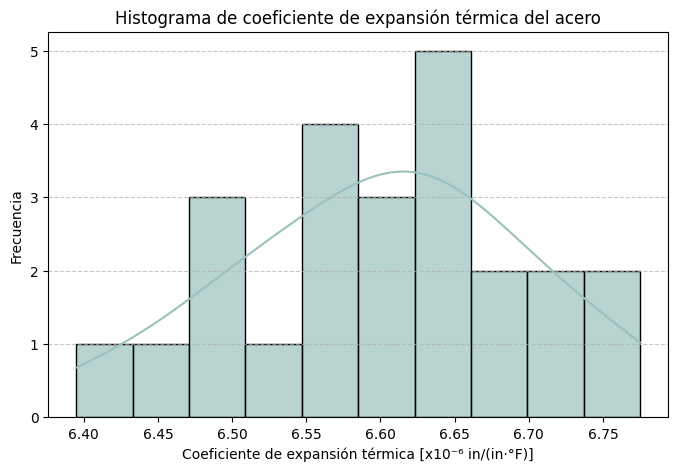
\includegraphics[width=0.5\linewidth]{img/histograma.png}
    \caption{Histograma de coeficiente de expansión térmica del acero.}
    \label{fig:histograma}
\end{figure}

%DISCUSIÓN
\newpage
\section{Discusión.}
Los resultados obtenidos proporcionan una visión detallada de la distribución y estabilidad del coeficiente de expansión térmica del acero.
\subsection{Análisis del Promedio y la Tendencia Central.}
El \textbf{valor medio} del coeficiente de expansión térmica del acero se ha calculado en $6.6 \times 10^{-6} \, \text{in}/(\text{in} \cdot {}^{\circ}F)$. Este valor es representativo del comportamiento térmico del material y puede utilizarse como referencia en cálculos de dilatación térmica y modelado de estructuras expuestas a variaciones de temperatura.
\subsection{Evaluación de la Dispersión y Variabilidad.}
La \textbf{desviación estándar} de $0.0971$ indica que la mayoría de los valores se encuentran cercanos a la media, lo que sugiere una \textbf{baja dispersión} en los datos. De manera complementaria, la \textbf{varianza} de $0.0094$ indica que los valores están muy cerca de la media, lo que significa que hay poca variación entre ellos. Esto sugiere que las mediciones son consistentes y estables, ya que no presentan grandes fluctuaciones, lo que permite confiar en la precisión del coeficiente de expansión térmica del acero.\\

Por otro lado, el \textbf{coeficiente de variación} ($CV = 1.47\%$)  indica que la dispersión relativa de los datos con respecto a su media es baja. Un CV menor al $5\%$ es generalmente interpretado como una \textbf{baja variabilidad}, lo que sugiere que el coeficiente de expansión térmica del acero es consistente y predecible.

\subsection{Interpretación del Histograma y Distribución de los Datos.}
El \textbf{histograma} generado permite visualizar la distribución de los valores del coeficiente de expansión térmica. Se observa que los datos se agrupan en torno a $6.6$ (siendo esta a su vez la media), con una disposición que sugiere una aproximación a la \textbf{distribución normal}. Cuando los datos siguen una distribución normal, la media coincide con el valor más frecuente, y la dispersión alrededor de esta se distribuye de manera simétrica. En este caso, la presencia de una curva suavizada sobre el histograma permitiría verificar si la forma de la distribución se ajusta a la normalidad.

Además, la \textbf{baja dispersión} de los valores sugiere que el coeficiente de expansión térmica del acero es un parámetro \textbf{estable}. Sin embargo, si se deseara un análisis más detallado, se podría evaluar la \textbf{asimetría} y el \textbf{coeficiente de curtosis} de los datos para determinar con mayor precisión su grado de normalidad.


\section{Conclusiones.}
El análisis realizado muestra que el coeficiente de expansión térmica del acero presenta una\textbf{ baja dispersión} y una \textbf{alta estabilidad}, lo que indica que sus mediciones son consistentes y predecibles. Esta estabilidad es crucial en aplicaciones de ingeniería, dónde el comportamiento térmico de los materiales influye en su rendimiento y seguridad.\\

La representación gráfica y los indicadores estadísticos confirman que los datos siguen una \textbf{distribución bien definida}, permitiendo su uso como referencia en el modelado térmico y la simulación de estructuras expuestas a variaciones de temperatura. Estos resultados destacan la fiabilidad del material.

%REFERENCIAS
\newpage
\section{Referencias.}
\begingroup
\renewcommand{\section}[2]{} 
\begin{thebibliography}{99}
    \bibitem{Palencia}
    Palencia, J. (s.f.). \textit{Histograma y Curvas de Distribución}. Universidad de Cantabria. Recuperado de \url{https://personales.unican.es/palencij/Documentos/HC_Tema_V.pdf}
    \bibitem{UV}
    Universidad de Valencia. (s.f.). \textit{Análisis estadístico con SPSS: Estadísticos descriptivos e inferenciales}. Recuperado de \url{https://www.uv.es/innomide/spss/SPSS/SPSS_0203a.pdf}
    \bibitem{UBA}
    Universidad de Buenos Aires. (2022). \textit{Apunte de Estadística para Métodos y Técnicas de la Física Experimental}. Recuperado de \url{https://materias.df.uba.ar/mytb2022c1/files/2022/03/Apunte_estad%C3%ADstica_2022.pdf}
\end{thebibliography}
\endgroup

%ANEXOS
\newpage
\section{Anexos.}
El código fuente y la implementación del taller en lenguaje Python pueden consultarse en el siguiente repositorio de GitHub: \noindent\url{https://github.com/mgonzalz/sn_talleres/blob/main/src/taller-01__promedios.ipynb}

\noindent A continuación, se presentan los fragmentos principales del código utilizado para la realización del taller.

\subsection{Código para el Cálculo de Parámetros Estadísticos.}
\noindent Para el cálculo de parámetros estadísticos, se han desarrollado dos versiones del mismo algoritmo:  

\begin{enumerate}
    \item \textbf{Implementación sin NumPy}. Utiliza únicamente funciones nativas de Python para calcular el promedio, la varianza, la desviación estándar y el coeficiente de variación. Si bien es funcional, puede ser menos eficiente en conjuntos de datos grandes.
        \begin{minted}[frame=lines, framesep=2mm, bgcolor=lightgray, fontsize=\small]{python}
        def calcular_estadisticas(x):  # x: lista de Python estándar
            N = len(x)
            media = sum(x) / N
            varianza = sum((xi - media) ** 2 for xi in x) / (N - 1)
            desviacion = (varianza) ** 0.5  # Sin usar np.sqrt
            cv = (desviacion / media) * 100 if media != 0 else float("NaN")
        
            return {
                "Promedio": media,
                "Desviación estándar": desviacion,
                "Varianza": varianza,
                "Coeficiente de variación (%)": cv
            }
        \end{minted}
    \item \textbf{Implementación con NumPy.} Aprovecha la optimización de las funciones de NumPy para realizar cálculos más rápidos y eficientes, especialmente útil en procesamiento de grandes volúmenes de datos. 
    \begin{minted}[frame=lines, framesep=2mm, bgcolor=lightgray, fontsize=\small]{python}
import numpy as np

def calcular_estadisticas_np(x):  # x: array de NumPy
    media = np.mean(x)
    varianza = np.var(x, ddof=1)
    desviacion = np.std(x, ddof=1)
    cv = (desviacion / media) * 100 if media != 0 else float("NaN")

    return {
        "Promedio": media,
        "Desviación estándar": desviacion,
        "Varianza": varianza,
        "Coeficiente de variación (%)": cv
    }
\end{minted}
\end{enumerate}

\newpage
\subsection{Código para la Carga, Análisis y Visualización de los Datos.}
Para analizar el coeficiente de expansión térmica del acero, se ha implementado un conjunto de funciones que permiten procesar y representar los datos de manera estructurada. Primero, se desarrolla una función encargada de leer y extraer los valores desde un archivo de texto, transformándolos en una lista numérica y asegurando que no contenga líneas vacías o datos incorrectos. Posteriormente, se genera un histograma con la curva de densidad utilizando la biblioteca Seaborn, lo que facilita la visualización de la distribución de los datos y permite evaluar si siguen una distribución normal.

\begin{minted}[frame=lines, framesep=2mm, bgcolor=lightgray, fontsize=\small]{python}
def leer_datos(archivo):  # archivo: ruta local del archivo str.
    try:
        with open(archivo, "r") as f:
            datos = [float(line.strip()) for line in f if line.strip()]
        if not datos:
            raise ValueError("El archivo está vacío o no contiene datos válidos.")
        return datos
    except Exception as e:
        print(f"Error al leer el archivo: {e}")
        return []
\end{minted}

\begin{minted}[frame=lines, framesep=2mm, bgcolor=lightgray, fontsize=\small]{python}
import matplotlib.pyplot as plt
import seaborn as sns

plt.figure(figsize=(8, 5))
sns.histplot(datos, bins=10, edgecolor='black', alpha=0.7, color='#9BC1BC', kde=True)
plt.ylabel("Frecuencia")
plt.xlabel("Coeficiente de expansión térmica [x10⁻⁶ in/(in·°F)]")
plt.title("Histograma de coeficiente de expansión térmica del acero")
plt.grid(axis='y', linestyle='--', alpha=0.7)
plt.show()
\end{minted}


\end{document}
